% set document class
\documentclass[letterpaper,man,natbib,longtable,floatsintext,12pt]{apa6}  

% load packages
\usepackage[english]{babel}
\usepackage[utf8x]{inputenc}
\usepackage{float}
\usepackage{amsmath}
\usepackage{graphicx}
\usepackage{booktabs}             % fancy latex tables
\usepackage[export]{adjustbox}    % center wide tables on page
\usepackage{setspace}             % adjust caption linespacing 
\usepackage{multibib}             % references in supplement
\usepackage{hyperref}             % manage hyperlink colors
\usepackage{hanging}

% override apa6 section headers
% https://tex.stackexchange.com/questions/125537/how-to-modify-subsubsection-header-apa6-cls
\makeatletter
\renewcommand{\subsubsection}{\@startsection{subsubsection}{3}
  {\z@}%
  {\b@level@two@skip}{\e@level@two@skip}%
  {\normalfont\normalsize\bfseries}}
\makeatother

% center contents of longtable
\usepackage{array}
\newcolumntype{P}[1]{>{\centering\arraybackslash}p{#1}}

% setup supplementary references
\newcites{SM}{Supplementary references}

% decrease size of references (lol)
\renewcommand*{\bibfont}{\small}

% change hyperlink colors
\hypersetup{
    colorlinks=true,
    linkcolor=blue,
    filecolor=magenta,      
    urlcolor=cyan,
    citecolor=blue
}

% define title page
\title{Evaluation of the factor structure and structural validity of the Maltreatment and Abuse Chronology of Exposure (MACE) scale}
\shorttitle{Structural validity of the MACE}
\author{Samuel Zorowitz$^{1*}$, Lauri Tuominen$^{2}$}
\affiliation{$^1$Princeton Neuroscience Institute, Princeton University, USA\\$^2$The Royal’s Institute of Mental Health Research, University of Ottawa, Canada\\$^*$Corresponding author: zorowitz@princeton.edu}

% add author note
\authornote{

{\begin{hangparas}{.25in}{1} \noindent Data availability: All data and analysis materials are publicly available at: \url{https://github.com/szorowi1/mace-irt}. \end{hangparas}}

{\begin{hangparas}{.25in}{1} Acknowledgments: The authors wish to thank Dr. Robyn McQuaid for thoughtful feedback on this manuscript. \end{hangparas}}

{\begin{hangparas}{.25in}{1} \noindent Ethics approval: The Institutional Review Board of the University of Ottawa (\#2021003) approved this study. \end{hangparas}}

{\begin{hangparas}{.25in}{1} \noindent Funding sources: This research was funded by the Royal's Emerging Research Innovators in Mental Health program at the University of Ottawa Institute of Mental Health Research and a National Science Foundation Graduate Research Fellowship. \end{hangparas}}

\noindent Conflict of interest: The authors have no conflicts of interest to declare.

}

% add abstract
\abstract{

\noindent \textbf{Purpose}: The Maltreatment and Abuse Chronology of Exposure (MACE) scale is a retrospective self-report measure of childhood maltreatment. Despite increasing use, the factor structure of the MACE has not been previously investigated. As such, the validity of the MACE total and subscale scores are unknown. The objective of the current study was to evaluate the factor structure of the MACE, including the structural validity of its total and subscale scores.

{\begin{spacing}{1.25} \hfill \\ \end{spacing}}

\noindent \textbf{Methods}: We analyzed the response data from two independent samples of participants who completed the MACE (N=1051 \& N=582) using confirmatory factor analysis. We fit a series of models of increasing dimensionality to explore its factor structure. We calculated model-based indices to quantify the reliability of the MACE total and subscale scores, and to test for essential unidimensionality. 

{\begin{spacing}{1.25} \hfill \\ \end{spacing}}

\noindent \textbf{Results}: Confirmatory factor analysis indicated that a bifactor S-1 model with two specific factors (peer victimization, reverse-scoring) provided the best and most parsimonious fit to the data. Model-based indices suggested the MACE scale is essentially unidimensional. The MACE total score was determined to be a reliable and valid measure of overall childhood maltreatment. In contrast, MACE subscale scores exhibited little reliable variance after controlling for overall maltreatment.

{\begin{spacing}{1.25} \hfill \\ \end{spacing}}

\noindent \textbf{Conclusions}: Our results suggest the MACE is essentially unidimensional and support the continued use of the MACE total score. However, our results caution against the use of MACE subscores, which provide little unique or reliable information above and beyond the total score.

{\begin{spacing}{1.15} \hfill \\ \end{spacing}}

}

\keywords{child maltreatment, reliability, item response theory, bifactor model}

\begin{document}

\maketitle

\section{Introduction}

Childhood maltreatment is a common experience \citep{stoltenborgh2015prevalence} that increases the risk for mental and physical illness  later in life \citep{kessler2010childhood, wegman2009meta} and predicts worse treatment response for multiple psychiatric disorders \citep{nanni2012childhood, thomas2019childhood}. Reliable and valid assessment of childhood maltreatment is an important research goal in order to better understand the link between maltreatment and health outcomes; improve treatment strategies for victims of childhood maltreatment; and design better interventions to prevent maltreatment before it occurs. 

There already exist many measures of childhood abuse and maltreatment for researchers to use \citep{saini2019systematic}. One recently developed measure, the Maltreatment and Abuse Chronology of Exposure scale (MACE; \citealt{teicher2015maltreatment}), has a number of notable advantages. First, the MACE measures 10 distinct types of childhood maltreatment, including four types that are seldom included in other scales (e.g., peer victimization, witnessing domestic violence). Second, the items in the MACE were selected using item response theory in order to ensure that each subscale assesses maltreatment experiences of increasing severity. Third, the MACE also measures the timing of maltreatment experiences, which is necessary for investigating how the chronology of abuse shapes development. Finally, the MACE total score (total number of unique maltreatment experiences) exhibits good psychometric properties, including excellent temporal stability, convergent validity with other childhood maltreatment scales, and predictive validity for many psychiatric symptoms \citep{teicher2015maltreatment}. For these reasons, the MACE has been appraised as among the best measures of childhood maltreatment currently available \citep{saini2019systematic, georgieva2022systematic}.

One critical issue for using the MACE in childhood maltreatment research is that its structural validity --- defined as the degree to which an instrument's scores adequately reflect the dimensionality of the construct being measured --- is unknown \citep{saini2019systematic}. This issue is pressing as some researchers have begun to use scores from each of the 10 MACE subscales to study the unique contributions of distinct maltreatment types to developmental outcomes (e.g., \citealt{schalinski2015type, gerke2018childhood, schalinski2019early}). Others have calculated bespoke subscale scores of threat and deprivation exposure using composites of MACE items that respectively measure abuse and neglect experiences (e.g., \citealt{schalinski2018defining, schalinski2019environmental, teicher2018differential}). Because the factor structure of the MACE has not been investigated, the validity of these subscale scores (i.e., the extent to which they reflect particular types of maltreatment as intended) is indeterminate.  

Though the MACE measures 10 distinct types of maltreatment, the factor structure that best explains the patterns of responses on the MACE may have fewer than 10 factors given the high co-occurrence of maltreatment experiences. That is, children who have experienced any single type of maltreatment are likely to have experienced multiple other types \citep{dong2004interrelatedness, herrenkohl2009assessing, kessler2010childhood}. As such, it is possible that MACE subscale scores may primarily reflect overall maltreatment rather than any specific type of maltreatment. Bifactor models, a type of hierarchical factor models, are well-suited for resolving this type of concern \citep{bornovalova2020appropriate}. Under a bifactor model, covariation in responses to a set of items are accounted for by a \emph{general} factor, reflecting shared variance across all items, and one or more \emph{specific} factors, reflecting additional shared variance among subsets of items \citep{Reise2012-ql}. Applied to the MACE, bifactor models can aid in determining whether its subscale scores are interpretable as measures of distinct types of maltreatment, or if they instead chiefly reflect general maltreatment. 

The main objective of the present study was to investigate the structural validity of the MACE. To do so, we fit a series of confirmatory factor models to the response data from two independent samples of participants who completed the MACE. The first objective of our analyses was to examine the dimensionality of the MACE; that is, to determine whether responses on the MACE are best-explained by a factor structure with 10 factors (one per subscale) or by a more parsimonious factor structure. The second objective was to quantify the reliability of, and sources of variability in, the MACE total and subscale scores in order to determine whether each score adequately measured its construct as intended. 

\section{Methods}

\subsection{Participants}

The participants in the current study (N=1633 total) belonged to one of two samples. The first sample of participants (N=1051) are from the original development of the MACE and the details of their recruitment have been reported elsewhere \citep{teicher2015maltreatment}. Briefly, inclusion criteria included being medically healthy, unmedicated, and between 18–25 years of age. This sample will hereafter be referred to as the \textit{original} sample. 

The second sample of participants (N=687) were recruited from Prolific Academic (\url{https://www.prolific.co}) to participate in an experiment in August -- October, 2021. Of these, N=582 were retained for analysis (see Exclusion Criteria below). Participants were eligible for participation if they were 18 years or older and resided in the United States or Canada. Participants received monetary compensation for their time (rate: \$12 USD/hr). This study was approved by the Institutional Review Board of the University of Ottawa (\#2021003), and all participants provided informed consent. This sample will hereafter be referred to as the \textit{replication} sample. 

The demographics of the samples are summarized in Table \ref{tab:demographics}. The majority of participants in both samples identified as women, but the original sample was composed of proportionally more woman ($z$ = 4.142, $p$ < 0.001). Participants in the original sample were also younger on average ($t$ = -19.313, $p$ < 0.001). The majority of participants identified as White and not as Hispanic or Latino. The proportion of participants identifying as White was not significantly different across samples ($z = 0.417$, $p = 0.677$), nor was the proportion of participants identifying as Hispanic or Latino ($z$ = -1.241, $p$ = 0.214).

\begin{table}[t!]
    \centering
    \begin{tabular*}{\textwidth}{lccc}
    \toprule
    Variable & Original (N=1051) & Replication (N=582) & p-value \\
    \midrule
    \textbf{Gender}, N (\%)                & & & p < 0.001 \\
    \hspace{1em} Women                     & 670 (63.7\%) & 310 (53.3\%) & \\
    \hspace{1em} Men                       & 381 (36.3\%) & 258 (44.3\%) & \\
    \hspace{1em} Transgender or nonbinary         &   0  (0.0\%) &   9  (1.5\%) & \\
    \hspace{1em} Rather not say            &   0  (0.0\%) &   5  (0.9\%) & \\
    \midrule
    \textbf{Age}, yrs                      & & & p < 0.001 \\
    \hspace{1em} Mean (range)              & 23.1 (18 -- 27) & 30.2 (18 -- 80) & \\
    \midrule
    \textbf{Ethnicity}, N (\%)             & & & p = 0.214 \\
    \hspace{1em} Not Hispanic or Latino    & 963 (91.6\%) & 518 (89.0\%) & \\
    \hspace{1em} Hispanic or Latino        &  84  (8.0\%) &  57  (9.8\%) & \\
    \hspace{1em} Rather not say            &   4  (0.4\%) &   7  (1.2\%) & \\
    \midrule
    \textbf{Race}, N (\%)                  & & & p = 0.677 \\
    \hspace{1em} White                     & 806 (76.7\%) & 441 (75.8\%) & \\ 
    \hspace{1em} Asian                     & 103  (9.8\%) &  65 (11.2\%) & \\
    \hspace{1em} Black or African American &  81  (7.7\%) &  31  (5.3\%) & \\
    \hspace{1em} Other                     &  61  (5.8\%) &  28  (4.8\%) & \\
    \hspace{1em} Rather not say            &   0  (0.0\%) &  17  (2.9\%) & \\
    \bottomrule
    \end{tabular*}
    \caption{\normalfont Demographics of the two samples included in this study. The original sample was recruited and reported by \cite{teicher2015maltreatment}. The replication sample was recruited by the current authors for the purposes of this study.}
    \label{tab:demographics}
\end{table}

\subsection{Measures}

All participants completed the 52-item version of the MACE \citep{teicher2015maltreatment}. The MACE is a retrospective self-report scale that measures 10 unique types of childhood maltreatment (i.e., parental verbal abuse, physical abuse, nonverbal emotional abuse, sexual abuse, emotional neglect, physical neglect, witnessing violence to siblings, witnessing interparental violence, peer verbal abuse, peer physical abuse). For each item, participants endorsed if they ever experienced a particular event during childhood (e.g., ``Parents or guardians intentionally pushed, grabbed, shoved, slapped, pinched, punched or kicked you'') and, if so, at what ages (up to age 18). Here we only analyze the dichotomous response data (Yes = 1, No = 0). Six of the 52-items --- evenly divided between the emotional and physical neglect subscales --- are reverse-scored (e.g., ``One or more individuals in your family helped you feel important or special''). For these items we followed the scoring procedure set by \cite{teicher2015maltreatment}: a score of 1 is assigned to a response only in the absence of a positive event for all 18 years of childhood. This is in contrast to all remaining items, where a score of 1 is assigned if maltreatment was experienced in at least one year of childhood.

In both the original and replication samples, participants completed a number of additional self-report symptom measures. We did not analyze these data and therefore do not discuss these measures further. For completeness, the additional self-report measures that were collected are reported in the Supplementary Materials. 

\subsection{Exclusion criteria}

To ensure data quality in the replication sample, we relied on attention checks embedded in the self-report measures to identify and remove participants engaging in inattentive responding (\citealt{zorowitz2021inattentive}; see the Supplementary Materials for details). The data from N=64 (9.9\%) participants were excluded for failing one or more attention checks, leaving the data from N=582 participants for analysis.

\subsection{Confirmatory item factor models}

To investigate the factor structure of the MACE, we tested four confirmatory item factor models. The basis of each model is the graded response model for ordered polytomous data \citep{samejima1997graded}. The factor structure for each model is depicted in Figure \ref{fig:models}. The first is a one-factor (undimensional) model where all items load onto a general maltreatment factor (Figure \ref{fig:models}a). The second is a bifactor model where all items load onto a general maltreatment factor and also one of 10 specific factors based on their subscale membership (Figure \ref{fig:models}b). We used this model to evaluate the reliability of the MACE subscale scores. 

The third model was motivated by previous research that used the MACE to calculate bespoke subscale scores measuring threat and deprivation experiences (e.g., \citealt{teicher2018differential}). To evaluate those scores, we initially fit a bifactor model where all items loaded onto a general maltreatment factor, and also a threat or neglect specific factor. After observing vanishing loadings on the threat specific factor, however, we instead fit a bifactor S-1 model \citep{eid2017anomalous} where all items loaded onto a general maltreatment factor, and only items measuring neglect load onto a specific neglect factor (Figure \ref{fig:models}c). We used this model to evaluate the reliability of the neglect subscale scores. 

\begin{figure}[t!]
    \centering
    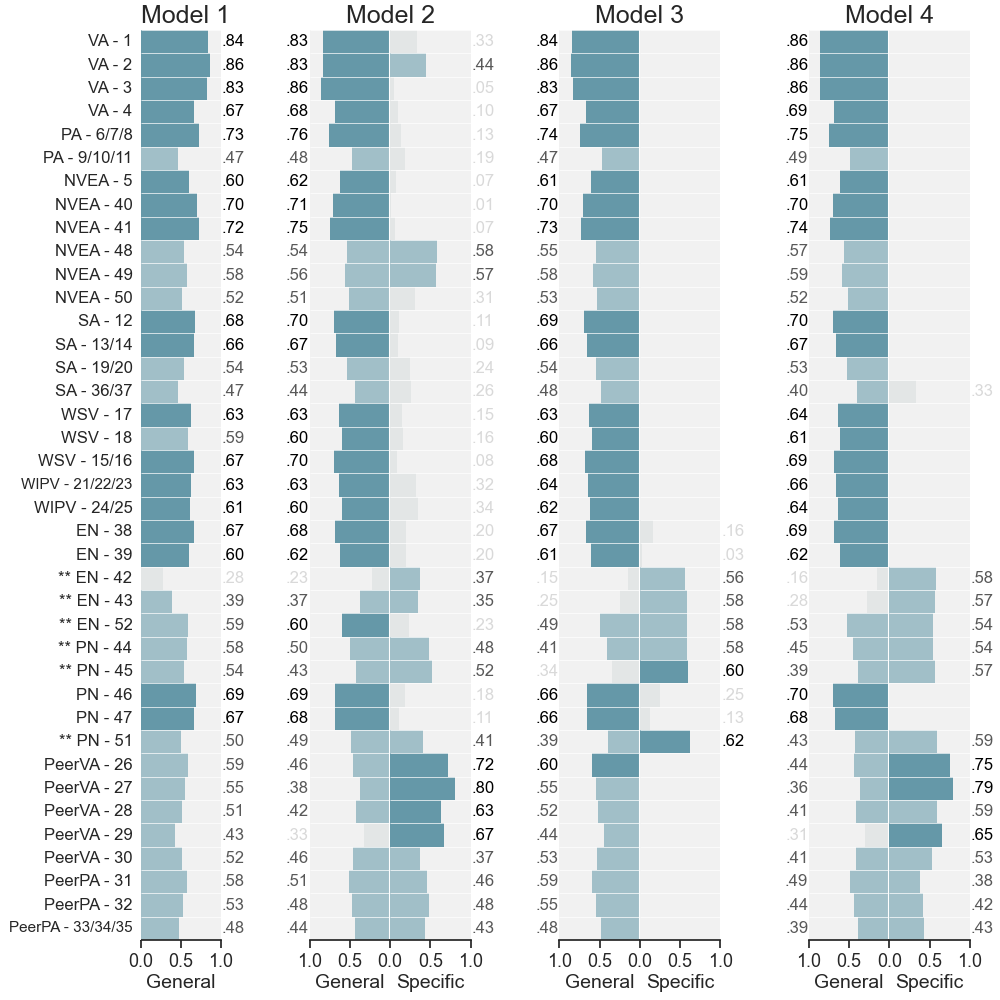
\includegraphics[width=1.1\textwidth,center]{figures/fig01.png}
    \captionsetup{width=1.1\textwidth}
    \caption{\normalfont The structure of the four competing confirmatory factor models of the MACE. (A) One-factor (unidimensional) model. (B) Bifactor model with 10 specific factors (one per MACE subscale). (C) Bifactor S-1 model with 1 specific factor (neglect). (D) Bifactor S-1 model with 2 specific factors (peer victimization, reverse-scored). Notes: G = general maltreatment; VA = verbal abuse; PA = physical abuse; NVEA = nonverbal emotional abuse; SA = sexual abuse; WSV = witnessing sibling vioence; WIPV = witnessing inter-parental violence; EN = emotional neglect; PN = physical neglect; PeerVA = peer verbal abuse; PeerPA = peer physical abuse.}
    \label{fig:models}
\end{figure}

The fourth model offers a more parsimonious structure of the MACE where items are organized according to the source of maltreatment: parents (or other adults in the home) and peers. That is, this model represents the hypothesis that two factors are sufficient to summarize responses on the MACE: a primary parental maltreatment factor and a secondary peer victimization factor. Based on preliminary model fits, we suspected the presence of a tertiary methods factor affecting the six reverse-scored items. We initially fit a bifactor model in which all items loaded onto a general maltreatment factor and one of three specific factors (i.e., parental maltreatment, peer victimization, reverse-scoring). After observing vanishing loadings on the first specific factor, however, we instead fit a bifactor S-1 model where all items load onto a general maltreatment factor, and the peer victimization and reverse-scored items additionally load onto their own specific factors (Figure \ref{fig:models}d). We fit this model to test a more parsimonious factor structure of the MACE, and to evaluate the reliability of peer victimization subscale scores. 

We fit each model separately to the data from the original and replication samples. We did so because, prior to analysis, we detected uniform differential item functioning (DIF) by sample for 11 items (see the Supplementary Materials for details). Also prior to analysis, we identified a total of 12 pairs and triplets of MACE items with response dependence. For example, a person endorsing item 8 (``Parents or guardians hit you so hard that you received medical attention'') is all but certain to endorse item 7 (``Parents or guardians hit you so hard that it left marks for more than a few minutes''). To prevent bias in the estimation of factor loadings due to response dependence \citep{reise2013applying}, we followed best-practice recommendations and combined each set of dependent items into a single polytomous item \citep{marais2008formalizing}. Thus, we reduced the MACE from 52 to 39 independent items (Table \ref{tab:dependence}).

All confirmatory item factor models were estimated within a Bayesian framework using Hamiltonian Monte Carlo as implemented in Stan (v2.26; \citealt{carpenter2017stan}). For each model, four separate chains with randomized start values each took 3,000 samples from the posterior. The first 2,000 samples from each chain were discarded, so that 4,000 post-warmup samples from the posterior were retained. The $\hat{R}$ values for all parameters were less than 1.01, indicating acceptable convergence between chains, and there were no divergent transitions in any chain. 

\subsection{Goodness of fit \& model comparison}

We relied on multiple indices to judge the fit of the models to the data. First we calculated three traditional goodness-of-fit statistics based on the ordinal $M_2$ statistic \citep{cai2013limited}. Specifically, we calculated the root mean square error of approximation (RMSEA), comparative fit index (CFI), and Tucker-Lewis index (TLI) for each model fit. Following convention \citep{hu1999cutoff}, we defined the benchmarks for adequate model fit as RMSEA < 0.08, CFI > 0.90, and TLI > 0.90, and the benchmarks for good model fit as RMSEA < 0.05, CFI > 0.95, and TLI > 0.95. 

Given the limitations of SEM-based fit indices for item response models (e.g., \citealt{clark2018model}), we calculated two additional fit indices. First, we used posterior predictive model checking to calculate a $\chi^2_{NC}$ discrepancy measure based on the total score distribution \citep{sinharay2006posterior}. This measure compares the observed and model-predicted proportion of participants at each total score level. Second, to test for local dependence in each pair of items, we calculated Yen's $Q_3$ statistic \citep{yen1984effects} and also the critical $Q_3$-value (i.e., the value above which local dependence is indicated; \citealt{christensen2017critical}). Briefly, for each model and sample, we simulated 1000 locally-independent datasets using the posterior distribution of model parameters. We then recorded the maximum $Q_3$ value per simulation. The critical $Q_3$-value was defined as the 99th percentile of these max $Q_3$ values. 

The goodness-of-fit of the models was compared using Bayesian leave-one-out cross-validation (LOO-CV; \citealt{vehtari2017practical}). LOO-CV quantifies the discrepancy between the model and data while taking into account model complexity. LOO-CV values are reported here in deviance scale (i.e., smaller values indicate better fit).

\subsection{Model-based reliability indices}

To evaluate the MACE total and subscale scores, we calculated several model-based reliability indices. First, we calculated coefficient omega ($\omega$; \citealt{mcdonald2013test}), which quantifies the proportion of reliable score variance attributable to all factors (i.e., both general and specific). Next we calculated coefficient omega hierarchical ($\omega_h$) and coefficient omega subscale ($\omega_s$;  \citealt{reise2013scoring}). Whereas $\omega_h$ measures the fraction of total score variance attributable to the general factor, $\omega_s$ measures the fraction of subscale score variance attributable to a specific factor. Larger values of $\omega_h$ indicate the general factor is the primary source of reliable variance in a total score. When $\omega_h > 0.80$, the total score is an essentially unidimensional reflection of the general factor \citep{rodriguez2016applying}. In turn, larger values of $\omega_s$ indicate the specific factor is the primary source of reliable variance in a subscale score. \cite{canivez2016bifactor} suggested that an acceptable $\omega_s$ value is 0.50 and that >0.70 is desirable. When $\omega_s < 0.50$, a subscale score instead primarily reflects the general factor \citep{gignac2013bifactor}. 

To evaluate the dimensionality of the MACE, we calculated the explained common variance (ECV; \citealt{sijtsma2009use}) and the proportion of uncontaminated correlations (PUC; \citealt{reise2013multidimensionality}). The ECV is the ratio of the variance explained by the general factor divided by the total common variance. It measures the contribution of the general factor relative to the specific factors. Larger ECV values indicate the general factor loadings of a bifactor model should resemble the loadings that would be obtained under a unidimensional model. When ECV > 0.70, a scale is essentially unidimensional \citep{rodriguez2016applying}. In turn, PUC quantifies how many inter-item correlations are accounted for only by the general factor. When PUC > 0.80, there is low risk of bias when a multidimensional scale is treated as unidimensional \citep{reise2013multidimensionality}. We also calculated the relative parameter bias (RPB), which is the difference between an item's loading in a unidimensional model and its corresponding general factor loading in a bifactor model, divided by the general factor loading from the bifactor model. RPB less than 10–15\% is acceptable \citep{muthen1987structural}.

We also calculated the H index \citep{hancock2001rethinking}, which measures how well a set of items represents a latent factor. Larger H values indicate a well-defined latent factor with item loadings more likely to be stable across studies. Because we are presently focused on evaluating the MACE total and subscale scores, we report H values but do not interpret them further.

\subsection{Exploratory factor analysis}

In addition to the confirmatory factor models, we also performed exploratory factor analysis (EFA) on each sample's data separately. The motivation for performing EFA was to examine whether any of the confirmatory factor structures emerged from the data with fewer \textit{a priori} restrictions \citep{schmitt2018selecting}. The details and results of the EFA are included in the Supplementary Materials. 

\section{Results}

\subsection{Goodness-of-fit \& model comparison}

The goodness-of-fit indices for each sample and model are summarized in Table \ref{table:cfa_diagnostics}. According to the traditional indices, each model provided at least an acceptable fit to the data. All RMSEA value were <0.05 and most CFI and TLI values were >0.95. The only exception were for the fits of models 1 and 3 to the original sample data where CFI and TLI > 0.90. Furthermore, none of the posterior predictive $p$-values from the $\chi^2_{NC}$ discrepancy measure exceeded the critical values, indicating that all models were able to reproduce the observed total score distribution for each sample.

Next we inspected the $Q_3$ indices for evidence of local dependence. For all models and samples, the maximum observed $Q_3$ index was greater than the critical $Q_3$ value. To measure the degree of local dependence, we visualized the $Q_3$ values for item pairs exceeding the critical value for each model and sample (Figure \ref{fig:local_dependence}). The unidimensional model fits exhibited many locally dependent item pairs, especially among the peer victimization and reverse-scored items, suggesting underfactorization. By comparison, the three bifactor models exhibited fewer locally-dependent item pairs. The cause for dependence among these item pairs were often self-evident. For example, the residual dependence between items 17 (``Parents made inappropriate sexual comments or suggestions to your sibling'') and 18 (``Parents touched or fondled your sibling in a sexual way'') is likely because these items measure similar content. Regardless, the estimated item discrimination parameters for each model fit seldom exceeded the normal range ($\alpha \leq 4$; \citealt{edwards2018diagnostic}); that is, the degree of local-dependence observed here did not result in substantial bias in parameter estimation. Thus, we conclude that all model fits provide at least an acceptable fit to the response data.

The results of the model comparison are also summarized in Table \ref{table:cfa_diagnostics}. Across samples, Models 2 and 4 provided better fits to the data than models 1 and 3. Model 2 provided a numerically better fit to the data than Model 4 in the original sample ($\Delta \text{LOO}$ = 7.9, se = 56.3), but the opposite was observed in the replication sample ($\Delta \text{LOO}$ = -24.0, se = 52.0). These differences in LOO-CV values, however, are both within four standard errors of the mean indicating only weak predictive improvements \citep{vehtari2022cv}. The results of the model comparison therefore suggest that Models 2 and 4 provide approximately equivalent fits to the data. This is noteworthy insofar that Model 4 assumes a substantially simpler factor structure of the MACE.

\begin{table}[t!]
\small
\centering
\begin{adjustbox}{center}
\begin{tabular}{ccccccccccr}
\toprule
Sample & Model & $\chi^2 (df)$ &  RMSEA & CFI & TLI & $\chi^2_{NC}$ (PPP) & $Q3_{\max}$ &  $Q3_{\text{crit}}$ & LOO-CV & \multicolumn{1}{c}{$\Delta$LOO (se)} \\
\midrule
Original & 1 &  1858 (702) &  0.040 &  0.927 &  0.923 &  0.051 (0.230) &  0.589 &  0.239 &  30967.2 &  1748.0 (76.7) \\
& 2 &  1373 (663) &  0.032 &  0.955 &  0.950 &  0.046 (0.356) &  0.573 &  0.300 &  29211.3 & \multicolumn{1}{c}{-} \\
& 3 &  1571 (692) &  0.035 &  0.944 &  0.940 &  0.051 (0.214) &  0.591 &  0.255 &  30531.1 &  1312.0 (68.0) \\
& 4 &  1253 (687) &  0.028 &  0.964 &  0.961 &  0.046 (0.346) &  0.591 &  0.279 &  29219.2 & 7.9 (56.3) \\
\midrule
Replication & 1 &  1086 (702) &  0.031 &  0.954 &  0.952 &  0.065 (0.629) &  0.513 &  0.250 &  19771.6 &  1089.3 (58.4) \\
& 2 &   956 (663) &  0.028 &  0.965 &  0.961 &  0.058 (0.766) &  0.456 &  0.310 &  18706.2 &    24.0 (52.0) \\
& 3 &   881 (692) &  0.022 &  0.977 &  0.976 &  0.062 (0.684) &  0.468 &  0.316 &  19177.7 &   495.5 (45.0) \\
& 4 &   842 (687) &  0.020 &  0.982 &  0.980 &  0.058 (0.756) &  0.437 &  0.318 &  18682.2 & \multicolumn{1}{c}{-} \\
\bottomrule
\end{tabular}
\end{adjustbox}
\captionsetup{width=1\textwidth}
\caption{\normalfont Fit statistics for the confirmatory factor models by sample. LOO-CV values are presented in deviance scale (i.e., smaller values indicate better fit). Notes: RMSEA = root mean square error of approximation; CFI = comparative fit index; TLI = Tucker-Lewis index; PPP = posterior predictive p-value; $Q3_{\max}$ = maximum $Q_3$ value in the sample for the model; $Q3_{\text{crit}}$ = critical $Q_3$ value for the model; LOO-CV = leave-one-out cross-validation.}
\label{table:cfa_diagnostics}
\end{table}

\subsection{Confirmatory item response models}

In the following, we interpret the fit of each confirmatory item response model. To facilitate interpretation, we have reproduced the standardized factor loadings of each model for the original sample in Figure \ref{fig:loadings_original} and for the replication sample in Figure \ref{fig:loadings_online}. The model-based reliability indices for the bifactor models are summarized in Table \ref{table:reliability}. 

\subsubsection{Model 1: One-factor (unidimensional) model}

The standardized factor loadings of the unidimensional model were, on average, large in magnitude. In the original sample, factor loadings ranged between 0.279 and 0.864 with an average value of 0.597 (95\% HDI = 0.579 -- 0.614); in the replication sample, factor loadings ranged between 0.359 and 0.814 with an average value of 0.600 (95\% HDI = 0.578 -- 0.621). Most items had loadings greater than 0.50 (original: 80.0\%, replication: 80.0\%), and therefore appear to be good indicators of general maltreatment. The rank correlation of general factor loadings between samples was $\rho$ = 0.565 (95\% HDI = 0.414 -- 0.711), indicating moderate agreement between samples.

In sum, the fits of the one-factor models provide partial evidence in support of a unidimensional model of the MACE. For example, most items exhibited moderate-to-large loadings on the unitary factor. However, the degree of local dependence present among in the unidimensional model fits (especially among the peer victimization items) suggest there may be secondary dimensions to the MACE. We turn next to the multidimensional confirmatory models to explore this possibility.

\begin{figure}[tp]
    \centering
    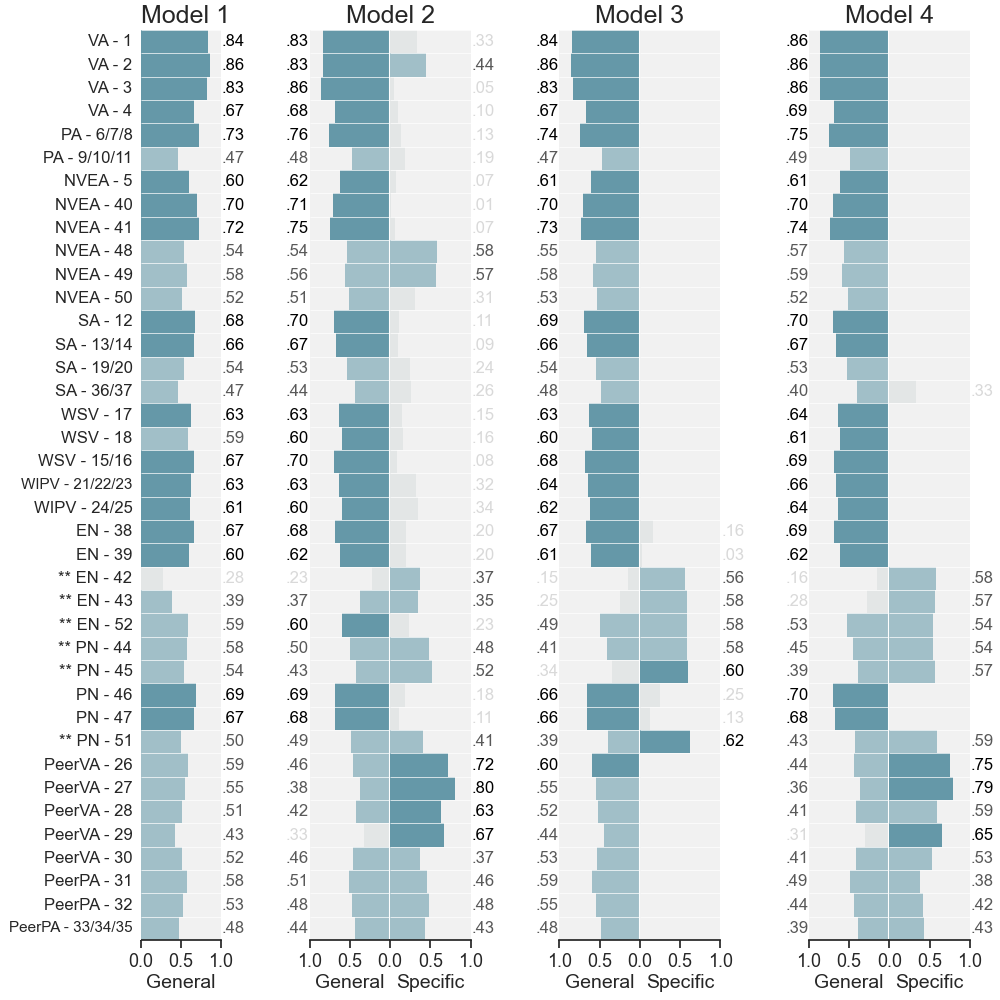
\includegraphics[width=1.1\textwidth,center]{figures/fig02.png}
    \captionsetup{width=1.1\textwidth}
    \caption{Standardized factor loadings from the four models fit to the original sample. Notes: Model 1 = one-factor (unidimensional) model; Model 2 = bifactor model with 10 specific factors; Model 3 = bifactor S-1 model with one specific factor (neglect); Model 4 = bifactor S-1 with two specific factors (peer victimization, reverse-scored); VA = verbal abuse; PA = physical abuse; NVEA = nonverbal emotional abuse; SA = sexual abuse; WSV = witnessing sibling vioence; WIPV = witnessing inter-parental violence; EN = emotional neglect; PN = physical neglect; PeerVA = peer verbal abuse; PeerPA = peer physical abuse. Factor loadings $<$ 0.3 are displayed in gray; factor loadings $\geq$ 0.6 are bolded.  ** Reverse-scored items.}
    \label{fig:loadings_original}
\end{figure}

\begin{figure}[tp]
    \centering
    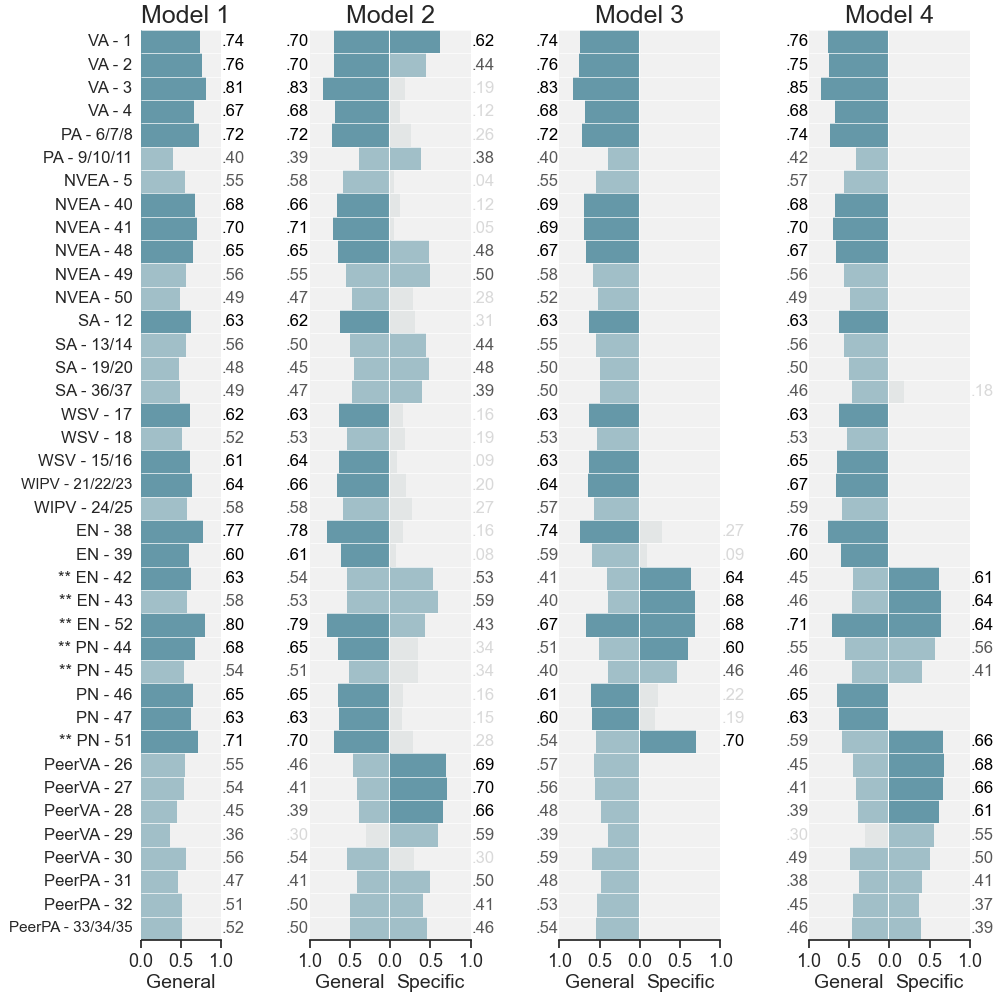
\includegraphics[width=1.1\textwidth,center]{figures/fig03.png}
    \captionsetup{width=1.1\textwidth}
    \caption{Standardized factor loadings from the four models fit to the replication sample. Notes: Model 1 = one-factor (unidimensional) model; Model 2 = bifactor model with 10 specific factors; Model 3 = bifactor S-1 model with one specific factor (neglect); Model 4 = bifactor S-1 with two specific factors (peer victimization, reverse-scored); VA = verbal abuse; PA = physical abuse; NVEA = nonverbal emotional abuse; SA = sexual abuse; WSV = witnessing sibling vioence; WIPV = witnessing inter-parental violence; EN = emotional neglect; PN = physical neglect; PeerVA = peer verbal abuse; PeerPA = peer physical abuse. Factor loadings $<$ 0.3 are displayed in gray; factor loadings $\geq$ 0.6 are bolded.  ** Reverse-scored items.}
    \label{fig:loadings_online}
\end{figure}

\subsubsection{Model 2: Bifactor model with 10 specific factors}

Next we inspect the bifactor model with 10 specific factors (i.e., one per MACE subscale). In the original sample, the loadings on the general maltreatment factor ranged between 0.235 and 0.864 with an average value of 0.575 (95\% HDI = 0.556 -- 0.593). In the replication sample, the general factor loadings ranged between 0.299 and 0.827 with an average value of 0.580 (95\% HDI = 0.560 -- 0.601). The relative parameter bias was marginal for both samples (original = 2.1\%; replication = 2.7\%), indicating an acceptable level of bias in the loadings of the one-factor models due to multidimensionality.  

In contrast, the loadings on the specific factors were small on average and rarely exceeded their corresponding loadings on the general factor. In the original dataset, the specific factor loadings ranged between 0.014 to 0.797 with an average value of 0.313 (95\% HDI = 0.285 -- 0.341). In the replication dataset, the range was between 0.043 and 0.698, with an average value of 0.343 (95\% HDI = 0.315 -- 0.369). Only items from the peer abuse subscales had specific factor loadings of greater magnitude to those on the general factor.

\begin{table}[t!]
\centering
\begin{tabular*}{\textwidth}{crccccccccc}
\toprule
& & & \multicolumn{4}{c}{Original} & \multicolumn{4}{c}{Replication} \\
\cmidrule(lr){4-7}\cmidrule(lr){8-11}
Model & Factor & PUC & ECV & $\omega$ & $\omega_{h/s}$ & H & ECV & $\omega$ & $\omega_{h/s}$ & H \\
\midrule
2 & General &  0.912 & 0.716 &  0.963 &   0.924 &  0.964 & 0.697 & 0.965 & 0.924 & 0.961 \\
& VA        &        &       &  0.909 &   0.069 &  0.273 &       & 0.893 & 0.162 & 0.478 \\
& PA        &        &       &  0.590 &   0.037 &  0.052 &       & 0.595 & 0.148 & 0.194 \\
& NVEA      &        &       &  0.848 &   0.136 &  0.525 &       & 0.827 & 0.117 & 0.424 \\
& SA        &        &       &  0.710 &   0.059 &  0.134 &       & 0.749 & 0.290 & 0.452 \\
& EN        &        &       &  0.715 &   0.162 &  0.304 &       & 0.874 & 0.203 & 0.542 \\
& PN        &        &       &  0.800 &   0.217 &  0.479 &       & 0.812 & 0.114 & 0.284 \\
& WSV       &        &       &  0.695 &   0.027 &  0.053 &       & 0.651 & 0.037 & 0.067 \\
& WIPV      &        &       &  0.655 &   0.146 &  0.197 &       & 0.612 & 0.077 & 0.107 \\
& PeerVA    &        &       &  0.878 &   0.621 &  0.818 &       & 0.853 & 0.565 & 0.766 \\
& PeerPA    &        &       &  0.699 &   0.335 &  0.443 &       & 0.694 & 0.337 & 0.446 \\
\midrule
3 & General &  0.939 & 0.864 &  0.958 &   0.928 &  0.964 & 0.841 & 0.959 & 0.922 & 0.959 \\
& Neglect   &        &       &  0.877 &   0.384 &  0.766 &       & 0.921 & 0.375 & 0.814 \\
\midrule
4 & General &  0.931 & 0.738 &  0.961 &   0.896 &  0.965 & 0.751 & 0.961 & 0.904 & 0.960 \\
& Peer      &        &       &  0.889 &   0.569 &  0.842 &       & 0.868 & 0.493 & 0.781 \\
& Reverse   &        &       &  0.839 &   0.584 &  0.739 &       & 0.915 & 0.498 & 0.773 \\
\bottomrule
\end{tabular*}
\captionsetup{width=1.\textwidth}
\caption{\normalfont Model-based reliability indices for the three bifactor models. Notes: PUC = proportion uncontaminated correlations; ECV = explained common variance; VA = verbal abuse; PA = physical abuse; NVEA = nonverbal emotional abuse; SA = sexual abuse; EN = emotional neglect; PN = physical neglect; WSV = witnessing sibling violence; WIPV = witnessing inter-parental violence; PeerVA = peer verbal abuse; PeerPA = peer physical abuse.}
\label{table:reliability}
\end{table}

The MACE total score had excellent reliability (original: $\omega$ = 0.963; replication: $\omega$ = 0.965). The $\omega_h$ value was 0.924 for both samples indicating that 96.0\% and 95.8\% of the reliable variance in the total score is attributable to general maltreatment. Importantly, the ECV values were 0.716 and 0.697 for the original and replication samples, respectively. Together with a PUC = 0.912, the ECV values suggest the MACE is essentially unidimensional. In sum, the results indicate the MACE total score is a reliable and structurally valid measure of overall maltreatment.

In turn, the reliability of the MACE subscale scores were smaller and more variable. The $\omega$ values ranged between 0.590 and 0.909 in the original sample, and between 0.595 and 0.893 in the replication sample. Most subscale scores exhibited at least adequate reliability ($\omega > 0.7$). Crucially, subscale scores contained little reliable variance after controlling for the general maltreatment factor (original: mean $\omega_s$ = 0.181, range = 0.027 -- 0.621; replication: mean $\omega_s$ = 0.205, range = 0.037 -- 0.565). That is, MACE subscale scores primarily reflect general maltreatment and not specific types of maltreatment. The only exception was for the peer verbal abuse subscale, where the majority of reliable variance in subscale scores was unique from general maltreatment (original = 70.7\%; replication = 66.2\%).

To summarize, the fits of the full bifactor model (Model 2) indicate responses on the MACE are largely explained by a general maltreatment factor with large loadings across items. In contrast, the specific factors corresponding to each MACE subscale were mostly characterized by small factor loadings. Whereas the MACE total score is a reliable and structurally valid measure of overall maltreatment, the majority of MACE subscale scores contain little reliable variance unique from general maltreatment. Thus, they cannot be said to reflect specific types of maltreatment. One question that remains, however, is if other reliable subscale scores can be derived from the MACE. 

\subsubsection{Model 3: Bifactor S-1 model with one specific factor (neglect)}

Next we inspect the bifactor S-1 model with one specific neglect factor (Model 3). The loadings on the general factor largely resembled those from Model 2. In the original sample, the loadings on the general maltreatment factor ranged between 0.150 and 0.864 with an average value of 0.577 (95\% HDI = 0.558 -- 0.594). In the replication sample, the general factor loadings ranged between 0.395 and 0.831 with an average value of 0.580 (95\% HDI = 0.558 -- 0.601). 

The loadings on the neglect specific factor were smaller on average. In the original sample, the average specific loading was 0.410 (95\% HDI = 0.373 -- 0.454); in the replication sample, it was 0.454 (95\% HDI = 0.409 -- 0.499). Troublingly, only the six reverse-scored items exhibited moderate loadings on the specific factor; the remaining four items exhibited negligible factor loadings. In other words, the ``neglect'' factor appears instead to reflect a reverse-scored methods factor.

The MACE total score exhibited excellent reliability (original: $\omega$ = 0.958; replication: $\omega$ = 0.959). Moreover, the $\omega_h$ values indicated the majority of reliable variance in severity score was attributable to the general factor (original: $\omega_h$ = 0.928; replication: $\omega_h$ = 0.922). The reliability of the ``neglect'' subscale score was also good (original: $\omega$ = 0.877; replication: $\omega$ = 0.921). As indicated by the $\omega_s$ values, however, reliable variance in the ``neglect'' subscale scores principally reflected the general maltreatment factor and not its intended construct (original: $\omega_h$ = 0.384; replication: $\omega_h$ = 0.375). 

In sum, the fits of Model 3 to the data do not support using the MACE to calculate independent threat and neglect subscale scores. As previously defined, the neglect subscale scores contain little reliable variance unique from general maltreatment and cannot, therefore, be said to measure neglect. Furthermore, most MACE items purportedly measuring neglect seem instead to reflect a reverse-scored methods artifact.

\subsubsection{Model 4: Bifactor S-1 with two specific factors (peer victimization, reverse- scoring)}

Finally, we inspect the bifactor S-1 model with two specific factors (peer victimization, reverse-scoring; Model 4). In the original sample, the loadings on the general maltreatment factor ranged between 0.158 and 0.864 with an average value of 0.563 (95\% HDI = 0.545 -- 0.580). In the replication sample, the general factor loadings ranged between 0.298 and 0.852 with an average value of 0.572 (95\% HDI = 0.550 -- 0.593). The loadings on the specific factors were similar in magnitude to those on the general factor. In the original dataset, the specific factor loadings ranged 0.327 to 0.789 with an average value of 0.550 (95\% HDI = 0.522 -- 0.576). In the replication dataset, the range was between 0.183 and 0.684 with an average value of 0.526 (95\% HDI = 0.492 -- 0.556). 

The MACE total score again exhibited excellent reliability (original: $\omega$ = 0.961; replication: $\omega$ = 0.961). Similarly, the majority of reliable variance in severity score was attributable to the general factor (original: $\omega_h$ = 0.896; replication: $\omega_h$ = 0.904). The peer victimization subscale scores exhibited good reliability across samples (original: $\omega$ = 0.889; replication: $\omega$ = 0.868). The corresponding $\omega_s$ values were 0.569 for the original sample and 0.493 for the replication sample indicating that the majority of variance in peer victimization scores were unique from the general maltreatment factor (original: 64.0\%; replication: 56.8\%). Thus, the results suggest (albeit weakly so) a secondary peer victimization factor in the MACE in addition to the general maltreatment factor. 

Briefly, we note that the subscale scores formed by the reverse-scored items were also reliable (original: $\omega$ = 0.839; replication: $\omega$ = 0.915). Moreover, the corresponding $\omega_s$ values were similar in magnitude to those observed for the peer victimization scores (original: $\omega_s$ = 0.584; replication: $\omega_s$ = 0.498). These scores therefore also exhibit majority reliable variance unique from general maltreatment. It is difficult to interpret these scores, however, as it is unclear what they primarily reflect (e.g., neglect, wording effects, reverse-scored methods artifact). 

\section{Discussion}

The MACE is a promising and increasingly popular measure of childhood maltreatment \citep{georgieva2022systematic}. Despite this, there has been no investigation into its factor structure \citep{saini2019systematic}, leaving unanswered questions about its structural validity and the interpretation of its total and subscale scores. Here we investigated the factor structure of the MACE through a series of confirmatory item response models. Our objectives were to evaluate the dimensionality of the MACE, and to quantify the degree and sources of reliable variance in its total and subscale scores. 

Of the confirmatory factor models we tested, the most parsimonious and best-fitting was the bifactor S-1 model with a general maltreatment factor and two smaller specific factors reflecting peer victimization and reverse item scoring (Model 4). This model provided a fit to the data equivalent to that for the more complex bifactor model with a specific factor for each MACE subscale. (This model was partially supported by EFA; see the Supplementary Materials for details.) Moreover, across all the models tested, a general maltreatment factor explained at least 70\% of the reliable variance in participants' responses. Together, the results support the conclusion that, while the content of the MACE is multidimensional, its factor structure is essentially unidimensional. 

We also found the MACE total score has excellent reliability. Given the essential unidimensionality of the MACE, the total score can be regarded as a valid and univocal index of overall childhood maltreatment. In stark contrast, we found that the majority of reliable variance for most MACE subscale scores was attributable to the general maltreatment and not specific types of maltreatment as intended. The same was true of the neglect subscale scores, which were additionally contaminated by a reverse-scored methods artifact. In sum, our results support the continued use of the MACE total score but caution against the use of MACE subscale scores. Indeed, the latter are unreliable measures of specific maltreatment types and instead predominantly reflect overall maltreatment. The only exception was the composite peer victimization subscale scores where the majority of reliable variance was attributable to the peer victimization factor and not general maltreatment. Regardless, additional research is needed to validate these subscores before they should be used in childhood maltreatment research.

Our results are consistent with previous studies that investigated the factor structure of other childhood maltreatment questionnaires. For example, bifactor models have revealed dominant general maltreatment factors and weaker specific factors for the Childhood Trauma Questionnaire \citep{spinhoven2014childhood, stagaki2022mediating}, International Child Abuse Screening Tool \citep{meinck2021factor}, and Adverse Childhood Experience questionnaire \citep{dobson2021latent}. Together, these and our results underscore a central challenge in childhood maltreatment research: when maltreatment experiences tend to co-occur, it is difficult to isolate the unique contribution of a particular type of adversity from overall maltreatment.
 
Our results are also worth considering alongside previous studies that used the MACE subscale scores to investigate the link between particular types of childhood maltreatment and assorted psychobiological outcomes. For example, researchers have looked at the relationship between MACE subscale scores and risk of depression \citep{gerke2018childhood}, dissociative symptoms, \citep{schalinski2015type}, and cortisol concentration \citep{schalinski2019early}. Still others have used bespoke threat and deprivation subscale scores from the MACE to study their associations with cognitive functioning \citep{schalinski2018defining} and hippocampal volume \citep{teicher2018differential}. Our results are unequivocal that these subscale scores mostly reflect general maltreatment and not particular types of adversity, which poses a challenge for interpreting the results of those studies. 

The current study revealed other features of the MACE worth highlighting. For example, we identified a number of items with DIF by sample. The cause for this is unclear and may reflect differences in sample populations, study locations, recruitment years, or inclusion/exclusion criteria. The causes and consequences of measurement noninvariance on the MACE deserve further study. We also identified a reverse-scoring methods factor in the MACE. The most plausible explanation for this is that, under the \cite{teicher2015maltreatment} scoring procedure, affirmative responses to the regular- and reverse-scored items on the MACE constitute very different answers. For a regular item on the MACE, an endorsement indicates that a person experienced an adverse event during at least one year of childhood. In contrast, an endorsement on a reverse-scored item indicates that a person experienced the absence of a positive event for all 18 years of childhood. However, alternative causes of this methods factor are plausible (e.g., participant confusion, acquiescence, or carelessness; \citealt{weijters2013reversed}). Further research is needed to see if alternative scoring procedures would mitigate this artifact. 

The current study is not without limitations. The most apparent limitation is that we only studied the dichotomous response data but not the chronology data that is also collected as part of the MACE. Though we found that the factor structure of the dichotomous responses is essentially unidimensional, this may belie more complex patterns present in the chronology data. Indeed, longitudinal models of adverse events across childhood (e.g., using dynamic factor analysis; \citealt{zhang2007bayesian}) might be more sensitive to patterns of maltreatment covariation that are lost when collapsing the data into simple yes/no responses. Another possibility is to jointly model the MACE endorsement and chronology data using a multidimensional hurdle model \citep{magnus2021symptom}, which measures both a person's susceptibility to maltreatment (number of maltreatment experiences) and severity of maltreatment (duration of maltreatment experiences). Further research is needed to develop maltreatment scores that jointly model the MACE endorsement and chronology data. 

A second limitation is our sample demographics. Though the replication sample increased the overall diversity of our sample with respect to gender and age, other types of diversity were notably lacking. Our combined sample was neither racially nor ethnically diverse. This is important as previous studies have identified DIF by race for other childhood adversity questionnaires \citep{rodriguez2019identification}. Additional research is needed to study the functioning of the MACE in more diverse samples in order to validate its use in those populations. 

To conclude, the results of the current study show the factor structure of the MACE is essentially unidimensional. Confirmatory bifactor models revealed that, despite the presence of smaller secondary factors, the majority of reliable variance in responses on the MACE is attributable to a general maltreatment factor. Accordingly, the MACE total score is a reliable and valid measure of overall childhood maltreatment. In contrast, the MACE subscale scores are invalid measures of their intended constructs; that is, they primarily reflect general maltreatment and not any specific type of maltreatment. Moving forward, we caution against the use of MACE subscale scores lest future childhood maltreatment researchers risk drawing invalid inferences. 

\bibliography{main}

\pagebreak
\section{Supplementary materials}

\setcounter{figure}{0}
\setcounter{table}{0}
\renewcommand{\thetable}{S\arabic{table}}
\renewcommand{\thefigure}{S\arabic{figure}}

\subsection*{Reflective vs. formative indicator models of maltreatment data}

One might question whether it is appropriate to explain childhood maltreatment data using common factor models with reflective indicators (e.g., bifactor models). The core assumption of these models is that variation in item responses are caused by or reflect variation in a shared latent factor (e.g., variation in low mood and anergia reflect latent individual differences in depression). This is in contrast to composite variable models with formative indicators where the direction of causality is reversed \citepSM{bollen1991conventional}. In composite variable models, indicators cause or form the latent construct (e.g., education and income together make up socioeconomic status). Some scholars have argued that measures of adverse childhood experiences should often be treated as formative, not reflective, indicators \citepSM{netland2001assessment, layne2010unpacking}. That is, exposure to abuse and neglect defines childhood maltreatment, not the other way around. 

For the purposes of explaining covariation in participants' responses on the MACE, we believe we are justified in using a common factor model. Most of the items on the MACE measure maltreatment by parents or other guardians. The homogeneity of these indicators suggests they might reflect a common source --- a hypothesis that is further supported by the uniformly strong (general) factor loadings we observed for this subset of items. Furthermore, there is ample theoretical and empirical support for regarding parental maltreatment as a common factor with its own causal antecedents \citepSM{belsky1993etiology}. Indeed, many of the same parent-level variables (e.g., emotional lability, impulse control, own history of abuse) are risk factors for different types of childhood maltreatment \citepSM{stith2009risk, mulder2018risk, assink2019risk}. 

Separately, that the MACE is a retrospective self-report measure is further justification for a common factor model. Retrospective measures of abuse have been shown to reflect additional factors beyond exposure to maltreatment including individual differences in current emotional state, personality, and recall ability \citepSM{susser2012still, reuben2016lest, colman2016consistency}. Common factor models are better suited to adjust the measurement error in indicators caused in part by these nuisance factors.

This discussion in turn raises a second question: is it reasonable for the items measuring parental maltreatment and peer victimization on the MACE to share a common factor? One might assume that these two types of maltreatment reflect independent causes and should therefore not be permitted to share a common factor. There is considerable evidence, however, that children who have been maltreated are at greater risk for subsequent peer victimization \citepSM{bolger2001developmental, benedini2016cycle}. The reasons for this association are manifold. For example, parental maltreatment may impact a child's sociocognitive functioning (e.g., attachment styles, emotion regulation) in ways that may predispose them to later peer victimization \citepSM{goemans2021child, McCrory2022-cj}. Separately, parental neglect is a risk factor for peer victimization \citepSM{lereya2013parenting}, possibly by increasing the chance that children enter into risky social situations where victimization may occur. Insofar that parental maltreatment is an indirect cause of peer victimization (mediated by multiple complex psychosocial pathways), then we believe we are justified in allowing indicators of peer victimization to load onto the common general maltreatment factor. This is also highlights the need for future study of MACE peer victimization subscale scores in order to better understand how it is similar to (and distinct from) parental maltreatment, and what their downstream sequalae are. 

\subsection*{Additional self-report measures}

In addition to the MACE, participants in both the original and replication samples completed a number of additional self-report measures. Participants in the original sample completed multiple measures of psychiatric symptoms, which have been reported elsewhere \citepSM{teicher2015maltreatment}. The participants in the replication sample completed three additional self-report measures assessing negative symptoms and motivation for rewards. Specifically, participants completed the Motivation and Pleasure scale \citepSM{llerena2013motivation}, the Self-evaluation of Negative Symptoms scale \citepSM{dollfus2016self}, and the revised Behavioral Inhibition / Behavioral Activation scale \citepSM{pagliaccio2016revising}.

Following best practices for online research \citepSM{zorowitz2021inattentive}, several attention checks were embedded in the secondary self-report measures filled out by the replication sample. Specifically, we used infrequency items which are questions for which all  or virtually all attentive participants should provide the same response. Specifically, we used the following questions:

\begin{enumerate}
    \item I'm able to blink my eyes without difficulty. (all endorse)
    \item I was motivated to write Mumfred Mumford's biography. (none endorse)
    \item I worry about the 2001 Cricket World Cup. (none endorse)
    \item Please select ``Yes'' and then select age ``17''. (instructed item)
\end{enumerate}

\noindent Prior to conducting the study, the infrequency items were piloted on an independent sample of participants to ensure that they elicited one dominant response. Participants were excluded from analysis if they responded incorrectly to one or more of these items.

\subsection*{Differential item functioning}

Prior to analysis, we investigated whether it was appropriate to combine response data from the original and replication samples. We first compared across samples the maltreatment endorsement rates for each item. The Spearman-rank correlation of endorsement rates across samples was large ($\rho$ = 0.951, p < 0.001), indicating excellent correspondence in the relative prevalence of maltreatment types across samples. When we compared the distribution of person-level total scores across samples, however, we found that scores were greater on average in the replication sample than in the original sample ($p_1$ = 0.185, $p_2$ = 0.219, $t$ = -4.611, p < 0.001). 

A mean shift in overall endorsement rates by sample is not necessarily evidence for a violation of measurement invariance. One possibility is that the replication sample had simply experienced more adversity than the original sample. A second is that the differences in the demographic composition of the two samples (e.g., gender, age) explain the differences in endorsement rates. To investigate these possibilities, we tested for uniform differential item functioning (DIF) using logistic regression, in which a participant's response on an item is regressed against their rest score (i.e., their total score for all other items), sample membership, gender, and age.

Using the cutoffs recommended by \citeSM{hidalgo2014binary}, we identified 11 of 52 items on the MACE with large DIF by study (Figure \ref{fig:dif_study}). These included all six reverse-scored items. We also found an additional 11 items with large DIF by gender (Figure \ref{fig:dif_gender}). Five of these items concerned sexual abuse (endorsed more frequently by women), and another five concerned peer physical abuse (endorsed more frequently by men). These findings are in line with previous research \citepSM{radford2013prevalence}. We identified no items that exhibited large DIF by age. Given the number of items with DIF by sample membership, we decided to analyze each sample separately.

\subsection*{Item response dependence}

Also prior to analysis, we found that the MACE contains a total of 12 item pairs and triplets characterized by response dependence (Table \ref{tab:dependence}). The items in some of these sets are structurally dependent, where a response to one item requires or strongly implies a certain response on the second. For example, a person endorsing item 8 (``Parents or guardians hit you so hard that you received medical attention'') is all but certain to endorse item 7 (``Parents or guardians hit you so hard that it left marks for more than a few minutes''). Other items are dependent by virtue of redundancy. One such example is items 36 (``Peers forced you to engage in sexual activity against your will'') and 37 (``Peers forced you to do things sexually that you did not want to do``); here the same question is asked twice using slightly different language.

Structurally-dependent or redundant items can cause serious problems for item factor models. First, they can inflate the estimates of item discrimination parameters, making items appear more reliable than they actually are \citepSM{marais2008formalizing}. Second, response dependence can cause overestimation of item loadings on specific factors in bifactor models, making specific factors (and subscores) appear more reliable than they actually are \citepSM{reise2013applying}. Following \citepSM{marais2008formalizing}, we therefore combined each set of dependent items into a single polytomous item thereby reducing the MACE from 52 to 39 items in total.

\subsection{Exploratory factor analysis}

In addition to confirmatory factor analysis, we also performed exploratory factor analysis (EFA) on the response data from each sample separately. The goal of the EFA was to examine what factor structure would emerge with no \emph{a priori} restrictions placed on the data. We decided to extract two- and three- factor solutions based on the total number of factors in the bifactor S-1 models. We were particularly interested to see if a two-factor solution would reproduce the factors from model 3 (threat, deprivation); and if a three- factor solution would reproduce the three factors from model 4 (parental maltreatment, peer victimization, reverse-scored). 

EFA was performed using the \textit{lavaan} (v0.6.11; \citealt{lavaan}) package available in R. Factors were extracted using the oblique geomin \citep{yates1987multivariate} and cf-quartimax rotation criteria \citep{crawford1970general}, which were selected in order to extract simple factor structures with few cross-loadings. We used two rotation criteria in order to examine the generalizability of the factor solutions across rotations. We again relied on traditional fit indices (i.e., RMSEA, CFI, TLI) to evaluate the goodness-of-fit of the exploratory factor models to the response data of both samples.

The goodness-of-fit measures for the exploratory factor models to the response data by sample are summarized in Table \ref{tab:efa_diagnostics}. The fit indices indicated that all exploratory models provided adequate fits to the data. The standardized factor loadings for the 2- and 3-factor solutions produced by the cf-quartimax rotation are presented in Figure \ref{fig:efa_cf}. The corresponding factor loadings produced by the geomin rotation were qualitatively similar and are presented in Figure \ref{fig:efa_geomin}. In the 2-factor solution for the original sample, we observed a primary parental maltreatment factor and a secondary peer victimization factor. In contrast, the replication sample produced an unclear factor solution characterized by strong loadings from the everse-scored items (F1) and peer victimization (F2). The parental maltreatment items then weakly loaded on both factors. Neither 2-factor solution precisely resembled the threat-deprivation factor structure of confirmatory model 3.

The 3-factor solutions for each sample were similar. EFA produced a primary parental maltreatment factor with secondary peer victimization and reverse-scored factors. Interestingly, items concerning sexual abuse loaded less strongly on the parental maltreatment factor in the replication sample, raising some questions about the replicability of the factor structures. Nevertheless, the structure of both the 2- and 3-factor exploratory factor models resembled most closely the bifactor S-1 model with two specific factors (model 4), providing further support for that model of the factor structure of the MACE. 

\pagebreak

\begin{longtable}{P{0.02\linewidth}p{0.7\linewidth}|P{0.05\linewidth}P{0.05\linewidth}P{0.05\linewidth}}
\centering
\# & Item & \multicolumn{3}{c}{Tetrachoric Corr.} \\
\toprule
6 & {\small Intentionally pushed, grabbed, shoved, slapped, pinched, punched or kicked you.} & - & & \\
7 & {\small Hit you so hard that it left marks for more than a few minutes.} & 0.778 & - &  \\
8 & {\small Hit you so hard, or intentionally harmed you in some way, that you received or should have received medical attention.} & 0.702 & 0.758 & - \\
\midrule
9& {\small Spanked you on your buttocks, arms or legs.} & - & \\
10	& {\small Spanked you on your bare (unclothed) buttocks.} & 0.862 & - & \\
11 & {\small Spanked you with an object such as a strap, belt, brush, paddle, rod, etc.} & 0.816 & 0.519 & - \\
\midrule
13 & {\small Touched or fondled your body in a sexual way.} & - \\
14 & {\small Had you touch their body in a sexual way.} & 0.954 & - \\
\midrule
15 & {\small Hit your sibling (stepsibling) so hard that it left marks for more than a few minutes.} &  \\
16 & {\small Hit your sibling (stepsibling) so hard, or intentionally harmed him or her in some way, that he/she received or should have received medical attention.} & 0.966 & - \\
\midrule
19 & {\small Had you touch their body in a sexual way.} & - \\
20 & {\small Actually had sexual intercourse (oral, anal or vaginal) with you.} & 0.909 & - \\
\midrule
21 & {\small Saw adults living in the household push, grab, slap or throw something at your mother (stepmother, grandmother).} & - \\
22 & {\small Saw adults living in the household hit your mother, stepmother, or grandmother so hard that it left marks for more than a few minutes.} & 0.920 & -  \\
23 & {\small Saw adults living in the household hit your mother, stepmother, or grandmother so hard, or intentionally harm her in some way, that she received or should have received medical attention.} & 0.808 & 0.934 & - \\
\midrule
24 & {\small Saw adults living in the household push, grab, slap or throw something at your father (stepfather, grandfather).} &  \\
25 & {\small Saw adults living in the household hit your father, stepfather, or grandfather so hard that it left marks for more than a few minutes.} & 0.900 & -\\
\midrule
33 & {\small Peers intentionally pushed, grabbed, shoved, slapped, pinched, punched, or kicked you.} & - \\
34 & {\small Peers hit you so hard that it left marks for more than a few minutes.} & 0.829 & - \\
35 & {\small Peers hit you so hard, or intentionally harmed you in some way, that you received or should have received medical attention.} & 0.723 & 0.907 & - \\
\midrule
36 & {\small Peers forced you to engage in sexual activity against your will.} &  - & \\
37 & {\small Peers forced you to do things sexually that you did not want to do.} & 0.975 & - \\
\bottomrule
\caption{\normalfont The 12 item pairs and triplets in the MACE characterized by response dependence. The tetrachoric correlation (averaged over samples) for each pair of items in a set is presented in tandem with the item wording.}
\label{tab:dependence}
\end{longtable}

\pagebreak

\begin{table}[H]
    \centering
    \begin{tabular}{llccccc}
    \toprule
    Sample      & Model    & $\chi^2$ ($df$) & RMSEA & CFI & TLI & SRMR \\
    \midrule
    Original    & 2-factor & 1876 (664) & 0.049 & 0.962 & 0.957 & 0.122 \\
                & 3-factor & 1237 (627) & 0.036 & 0.981 & 0.977 & 0.105 \\
    \midrule
    Replication & 2-factor & 1612 (664) & 0.051 & 0.961 & 0.957 & 0.121 \\
                & 3-factor & 1100 (627) & 0.037 & 0.981 & 0.977 & 0.111 \\
    \bottomrule
    \end{tabular}
    \caption{\normalfont Fit statistics for the exploratory factor models by sample. Notes: RMSEA = root mean square error of approximation; CFI = comparative fit index; TLI = Tucker-Lewis index; SRMR = standardized root mean square residual.}
    \label{tab:efa_diagnostics}
\end{table}

\pagebreak

\begin{figure}[H]
    \centering
    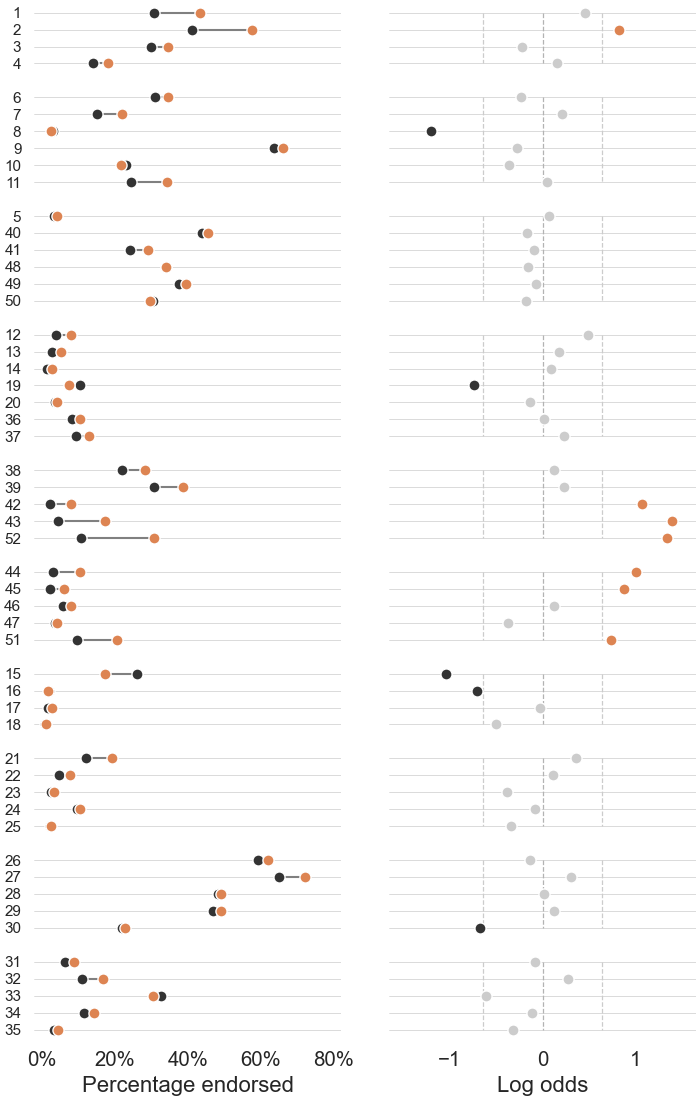
\includegraphics[width=0.82\textwidth,center]{figures/figS01.png}
    \caption{\normalfont Differential item functioning by sample. (A) Proportions of participants that endorsed experiencing a maltreatment event by study sample. (B) The log-odds that the proportion of endorsements are larger in one group. Dotted lines indicate the threshold for large DIF recommended by \cite{hidalgo2014binary}. ** Reverse-scored items.}
    \label{fig:dif_study}
\end{figure}

\pagebreak

\begin{figure}[H]
    \centering
    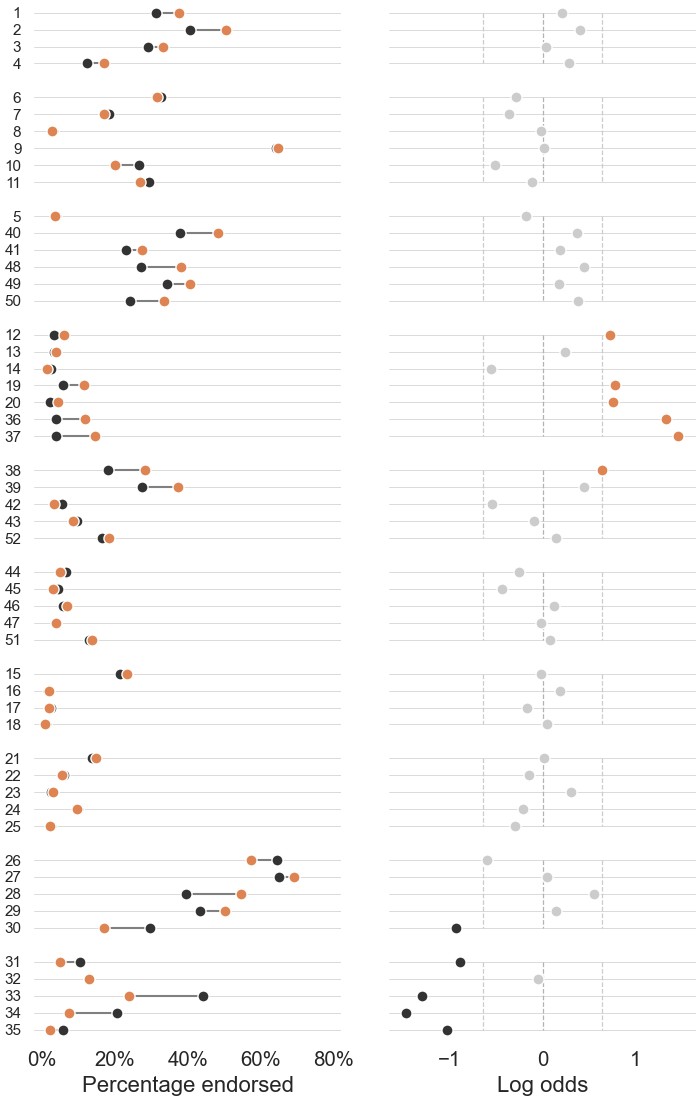
\includegraphics[width=0.82\textwidth,center]{figures/figS02.png}
    \caption{\normalfont Differential item functioning by gender. (A) Proportions of participants that endorsed experiencing a maltreatment event by gender. (B) The log-odds that the proportion of endorsements are larger in one group. Dotted lines indicate the threshold for large DIF recommended by \cite{hidalgo2014binary}. ** Reverse-scored items.}
    \label{fig:dif_gender}
\end{figure}

\pagebreak

\begin{figure}[H]
    \centering
    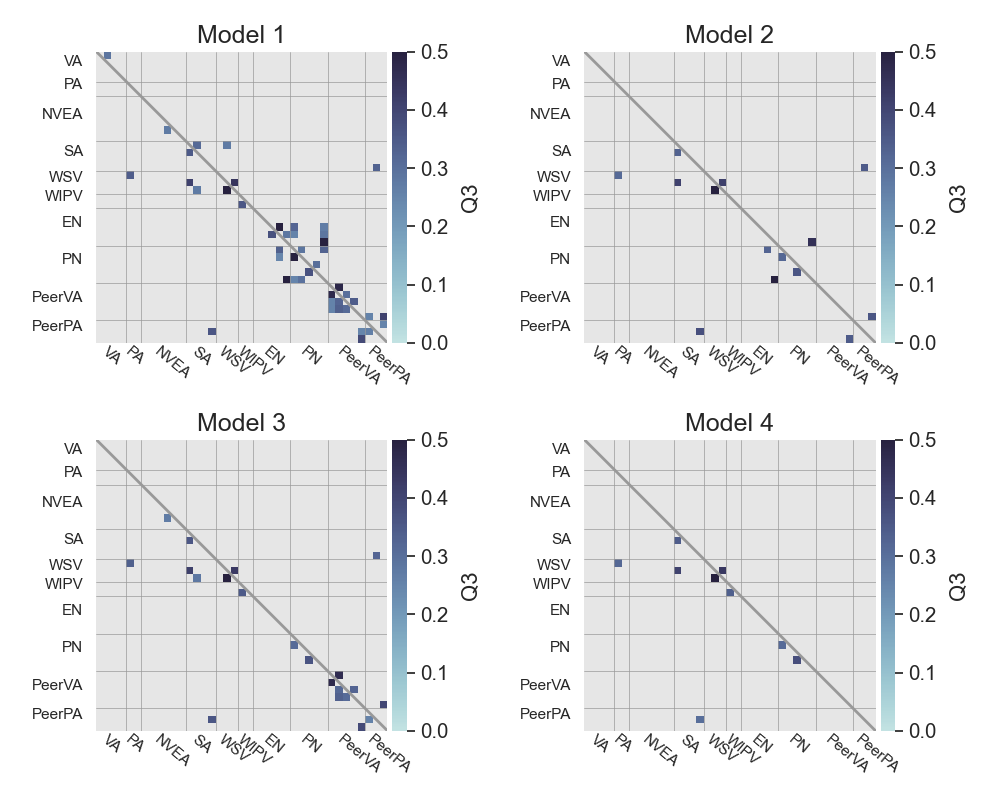
\includegraphics[width=1.05\textwidth,center]{figures/figS03.png}
    \caption{\normalfont Yen's $Q_3$ values for item pairs exceeding the 99\% percentile critical value for each confirmatory item response model. Cells beneath the gray diagonal line correspond to the original sample, whereas cells above the line correspond to the replication sample. Notes: VA = verbal abuse; PA = physical abuse; NVEA = nonverbal emotional abuse; SA = sexual abuse; EN = emotional neglect; PN = physical neglect; WSV = witnessing sibling violence; WIPV = witnessing inter-parental violence; PeerVA = peer verbal abuse; PeerPA = peer physical abuse.}
    \label{fig:local_dependence}
\end{figure}

\pagebreak

\begin{figure}[H]
    \centering
    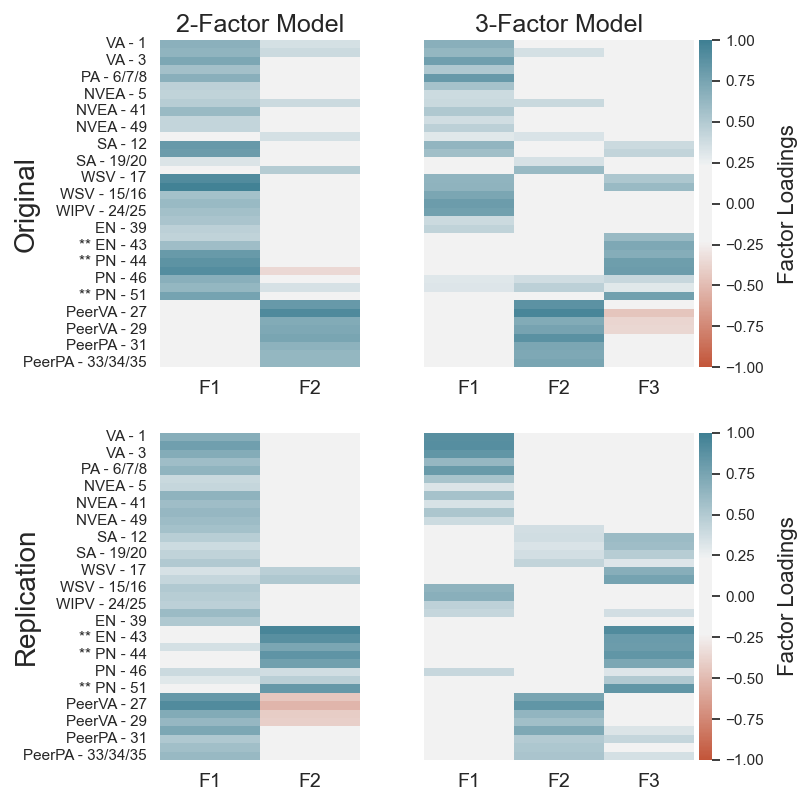
\includegraphics[width=1\textwidth,center]{figures/figS04.png}
    \caption{\normalfont Standardized factor loadings for the 2- and 3-factor solutions produced by the cf-quartimax rotation for original sample (top row) and replication sample (bottom row). \break \small Notes: VA = verbal abuse; PA = physical abuse; NVEA = nonverbal emotional abuse; SA = sexual abuse; EN = emotional neglect; PN = physical neglect; WSV = witnessing sibling violence; WIPV = witnessing inter-parental violence; PeerVA = peer verbal abuse; PeerPA = peer physical abuse. Only factor loadings $\geq$ 0.30 are shown. ** Reverse-scored items.}
    \label{fig:efa_cf}
\end{figure}

\pagebreak

\begin{figure}[H]
    \centering
    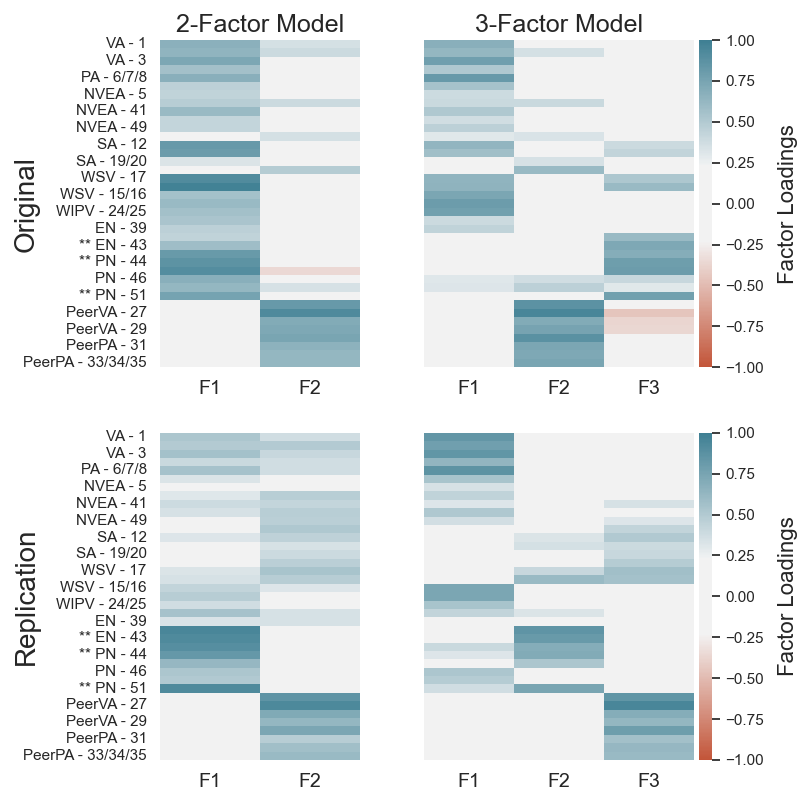
\includegraphics[width=1\textwidth,center]{figures/figS05.png}
    \caption{\normalfont Standardized factor loadings for the 2- and 3-factor solutions produced by the geomin rotation for original sample (top row) and replication sample (bottom row). Notes: VA = verbal abuse; PA = physical abuse; NVEA = nonverbal emotional abuse; SA = sexual abuse; EN = emotional neglect; PN = physical neglect; WSV = witnessing sibling violence; WIPV = witnessing inter-parental violence; PeerVA = peer verbal abuse; PeerPA = peer physical abuse. Only factor loadings $\geq$ 0.30 are shown. ** Reverse-scored items.}
    \label{fig:efa_geomin}
\end{figure}

\pagebreak

\bibliographystyleSM{apalike}
\bibliographySM{main}

\end{document}
